\chapter{Fundamentação Teórica}
\label{cap2}



\section{Jogos Eletrônicos}



O primeiro sistema de entretenimento interativo foi construído em 1947, utilizando como base de exibição um tubo de raios catódicos.
%
Essa criação foi patenteada em janeiro de 1948, datando então o início dos jogos eletrônicos~\cite{Adams2014Jan, patents1947Jan}.



O jogo eletrônico, ou entretenimento interativo, é uma atividade intelectual que integra um sistema de regras, na qual utiliza tal sistema a fim de definir seus objetivos ou pontuação por meio de um computador com o objetivo de despertar alguma emoção ao jogador~\cite{video_game_technologies}.
%
Os jogos eletrônicos são aplicações convencionais, que executam sobre algum sistema operacional ou hardware apropriado a este fim.
%
O sistema operacional, hardware ou base de execução da aplicação gráfica define a sua plataforma (\textit{e.g.,} GNU/Linux, MS-Windows, Sony PS4, MS-XBox, web, etc.)~\cite{adams_1208533}.



Inicialmente os jogos eram implementados de forma simples por conta da limitação de hardware das plataformas dos anos 80.
%
As implementações de jogos para \textit{videogames} eram desenhadas diretamente para algum hardware proprietário, sem sistema operacional, por muitas vezes sem utilizar comunicação por rede ou memória de disco~\cite{rollings2003andrew}.
%
Além de diversas plataformas não terem acesso a rede, os serviços para jogos eram inviabilizados pelo custo de manutenção e pela ausência de demanda a qual teriam os requisitos mínimos para jogar~\cite{adams_1208533}.
%
Na década de 80, o \textit{videogame} Atari foi uma plataforma popular, vendendo 30.000 unidades em seu lançamento contra apenas 2.000 unidades do seu concorrente Intellivision~\cite{atari_age}.



O crescente recurso computacional disponível em computadores pessoais e \textit{videogames} após os anos 90 permitiu que desenvolvedores criassem novos estilos de jogos que utilizavam de hardware mais especificado~\cite{adams_1208533}.
%
Dentre esses hardwares, iniciou-se o uso da rede de computadores para prover a interação entre jogadores de máquinas distintas~\cite{statisita_consumo_rede}.
%
Jogos como EA Habitat\footnote{EA Habitat: \url{http://www.mobygames.com/game/c64/habitat/credits}}, CipSoft Tibia\footnote{CipSoft Tibia: \url{http://www.tibia.com/}} e Jajex Runescape\footnote{Jajex Runescape: \url{https://www.runescape.com}} começam a utilizar, como requisito obrigatório do jogo, a conexão com a Internet para interagir em um mundo compartilhado com outos jogadores.
%
Tais jogos popularizaram um novo gênero, trazendo inovação em sua de jogabilidade e desafio proposto ao jogar com milhares de jogadores~\cite{guinness_runescape, 1417630}, criando o gênero de jogos \ac{mmo} na árvore de gêneros.



Nesse sentido, as redes de computadores serviram como impulsionador para várias categorias de jogos que antes não eram possíveis por conta da limitação de comunicação entre computadores.
%
Sendo assim, torna-se necessário ter uma visão geral das principais categorias de jogos eletrônicos.



\subsection{Árvore de gêneros de jogos eletrônicos}
\label{sec:arvore_generos}


A classificação por gênero é uma ferramenta tradicional para auxiliar a fácil identificação de características de alguma literatura, arte e outras mídias.
%
Dentro de jogos eletrônicos, o gênero permite que jogadores comprem jogos com características próximas conforme o seu gosto~\cite{Clarke2015}.



\begin{figure}[htb!]
\caption{Árvore de gêneros de jogos eletrônicos simplificada.}
\label{fig:generos}
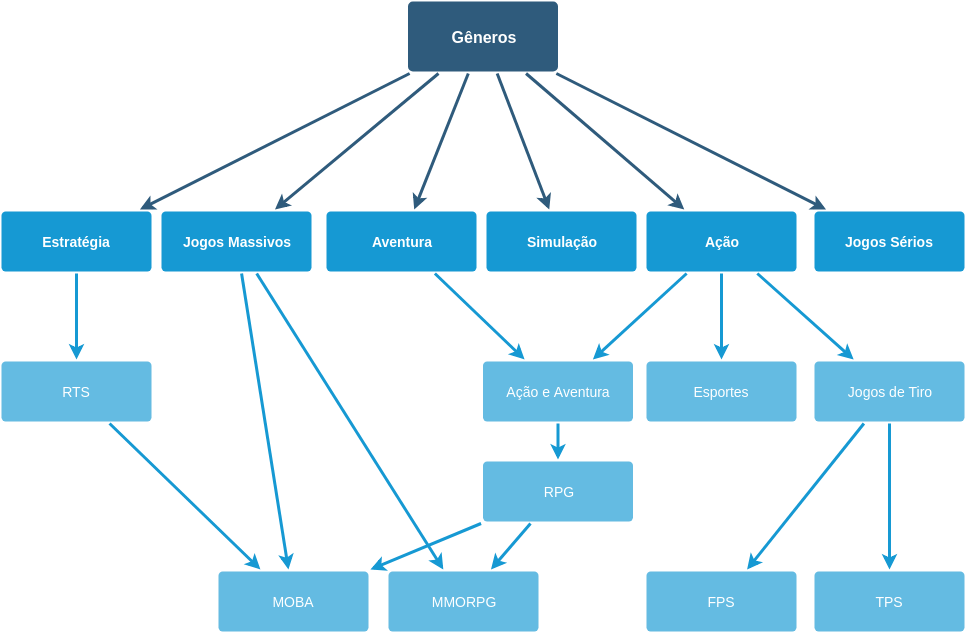
\includegraphics[height=9cm]{img/cap2/generos.png}
\centering

Adaptado de:~\cite{adams_1208533}
\end{figure}



Um gênero de jogo eletrônico é uma categoria específica para agrupar estilos de jogabilidade parecidos.
%
Porém, gêneros não definem de forma explícita o conteúdo expresso em algum jogo eletrônico, mas sim um desafio comum presente no jogo analisado~\cite{adams_1208533, video_game_technologies}.
%
Cada gênero de jogo contém variações, para uma melhor classificação.
%
A árvore pode ser visualizada pelo diagrama na Figura \ref{fig:generos}.
%
O contexto breve de cada gênero é:



\begin{itemize}
  \item Estratégia: São focados em uma jogabilidade que exija habilidades de raciocínio e/ou gerenciamento de recurso. Neste gênero, o jogador tem uma boa visualização do mundo, controlando indiretamente as suas tropas disponíveis~\cite{rollings2003andrew}. É comum encontrar jogos que disponibilizam algum modo de competição entre jogadores usando \ac{lan}, \ac{wan} ou \ac{p2p}~\cite{adams_1208533}.
    \begin{itemize}
      \item \ac{rts}: Utiliza as características de um jogo de estratégia, porém esse subgênero indica que as jogadas dos jogadores não são atômicas. É comum encontrar modos de jogo competitivo utilizando \ac{lan} neste gênero~\cite{adams_1208533}.
    \end{itemize}
  \item \ac{mmo}: Preza pela interação com outros jogadores em um mundo compartilhado~\cite{adams_1208533}. SecondLife\footnote{SecondLife: \url{https://www.secondlife.com/}} é um jogo focado na interação social, com artifícios de comércio e relacionamentos em um mundo fictício criado pela comunidade~\cite{tecmundo_secondlife}. Em grande parte, esses jogos utilizam tecnologia \ac{wan} e \ac{ws}.
    \begin{itemize}
      \item \ac{moba}: Coloca um número fixo de jogadores separados em dois times, no qual o time com maior estratégia de posicionamento e gerenciamento de recursos em equipe ganha a partida. Jogos \ac{moba} perdem algumas características breves do gênero \ac{rpg}, deixando de lado a interpretação e contextualização de um mundo, fixando-se somente em um combate estratégico e momentânio (distribuído em partidas átomas) entre as equipes, carregando consigo somente as características de comércio e comunidade dos jogos \ac{mmo}~\cite{adams_1208533}. Tal subgênero é popularmente conhecido pelos títulos Blizzard Dota 2\footnote{Blizzard Dota 2: \url{http://br.dota2.com/}} e Riot League of Legends\footnote{Riot League of Legends: \url{https://br.leagueoflegends.com/pt/}}. O jogo League of Legends obteve 100 milhões de usuários ativos em 2016~\cite{lol_statista}, além de ter um torneio nacional e mundial~\cite{lol_sportv}. É popular nesse subgênero utilizar tecnologias como \ac{lan}, \ac{p2p} e \ac{wan}.
      \item \ac{mmorpg}: Herda características dos gêneros ação e aventura, \ac{rpg}, e \ac{mmo} diretamente. Nesse gênero se faz permitido interações em um mundo na qual outros jogadores também estão jogando, na qual a interação entre outros jogadores (herdado dos jogos \ac{mmo}), com o mundo (herdado dos jogos de ação e aventura) e com objetivos guiados por \ac{npcs} (herdados de jogos \ac{rpg}) se faz como desafio e objetivo do jogo~\cite{adams_1208533}. Um título popular para esse gênero é o jogo Word of WarCraft\footnote{Word of WarCraft: \url{https://worldofwarcraft.com/pt-br/}}. A grande parte dos jogos \ac{mmorpg} utilizam tecnologia \ac{wan}.
    \end{itemize}
  \item Aventura: Caracterizado por desafios envolvendo ações com diversos \ac{npcs} ou com o ambiente para solucionar desafios~\cite{adams_1208533}. A grande parte desses jogos utilizam arquiteturas \ac{wan}, \ac{p2p} ou \ac{lan}.
    \begin{itemize}
      \item Ação e Aventura: Herda características da categoria de Ação e Aventura. O jogador é imerso em um mundo para iteragir com o ambiente e com \ac{npcs}, além de se preocupar com a movimentação no cenário~\cite{adams_1208533}. Um título popularmente conhecido desse gênero é a série de jogos nomeada Nintendo The Legend of Zelda\footnote{Nintendo The Legend of Zelda: \url{https://www.zelda.com/}}. É comum nesses jogos encontrar tecnologia \ac{lan} ou \ac{p2p} para modo de jogo cooperativo.
    \end{itemize}
  \item Simulação: Caracterizados por abordar temas da realidade. São comuns jogos de construção e gerenciamento, animais de estimação, vida social e simulação de veículos~\cite{adams_1208533}. A grande parte desses jogos não permite a interação entre os demais jogadores. É popular encontrar serviços como \textit{ranking}, loja e janela de notícias utilizando \ac{ws}.
    \begin{itemize}
      \item Esportes: Trata somente da simulação de esportes, nos quais o(s) time(s) podem ser controlados tanto por uma inteligência artificial quanto por jogadores online~\cite{adams_1208533}. O jogo FIFA\footnote{FIFA: \url{https://www.easports.com/br/fifa}} é um título popular nesse segmento. É comum encontrar tecnologias \ac{p2p} e \ac{lan}.
    \end{itemize}
  \item Ação: Preza pela habilidade de coordenação motora e reflexos do jogador, para tomar uma atitude a fim de passar seus objetivos no cenário. Nesse gênero os objetivos são passar por uma série de desafios que incluam movimentação e posicionamento de outros objetos no cenário~\cite{adams_1208533}. É comum encontrar tecnologias \ac{lan}, \ac{p2p}, \ac{wan} e \ac{ws}.
    \begin{itemize}
      \item Jogos de Tiro: Usa um número finito de armas para executar ações a distância. O posicionamento, movimentação estratégia e mira são fatores de desafio ao jogador nesse gênero~\cite{adams_1208533}. É comum encontrar tecnologias \ac{lan}, \ac{p2p} ou \ac{wan}.
        \begin{itemize}
          \item \ac{fps}: Utiliza o método de gravação conhecido como \ac{pov}. Nesse método, o modo de exibição do mundo é dado como a visão de um personagem do jogo, na qual o jogador tem visão pelo próprio personagem~\cite{video_game_technologies, adams_1208533}. É comum encontrar tecnologias \ac{lan}, \ac{p2p} ou \ac{wan}.
          \item \ac{tps}: Diferente dos jogos \ac{fps}, os jogos \ac{tps} utilizam cameras soltas no cenário no qual o jogador é visível na cena exibida~\cite{video_game_technologies, adams_1208533}. É comum encontrar tecnologias \ac{lan}, \ac{p2p} ou \ac{wan}.
        \end{itemize}
    \end{itemize}
  \item Jogos sérios: Tem como objetivo transmitir um conteúdo educacional~\cite{video_game_technologies}. O jogo Sherlock Dengue 8~\cite{sherlock_dengue} é um título desenvolvido com o objetivo de conscientizar os problemas e a prevenção da Dengue no Brasil. É comum encontrar tecnologias \ac{lan}, \ac{p2p}, \ac{wan} e \ac{ws}.
\end{itemize}



Dentre vários gêneros, alguns utilizam popularmente algumas tecnologias de rede.
%
A Tabela~\ref{tab:comunicacao_genero} indica a correlação de tecnologias de rede comuns nos gêneros, além de trazer a correlação de número de jogadores por gênero de jogo.
%
Essa correlação é importante para identificar as características de jogabilidade referente a jogabilidade com multijogadores~\cite{video_game_technologies}.


\begin{table}[htb!]
\centering
\caption{Tipos de comunicação e quantia de jogadores populares em gêneros}
\label{tab:comunicacao_genero}
\begin{tabular}{|l|l|l|l|l|l|}
\hline
                & \ac{lan}   & \ac{p2p}   & \ac{wan}            & \ac{ws}  &  Jogadores                                            \\ \hline
ESTRATÉGIA      & \checkmark & \checkmark & \checkmark         &              &   até 10~\cite{eoe3}                              \\ \hline
RTS             & \checkmark &            &                    &              &   até 10~\cite{starcraft2}                        \\ \hline
MMO             &            &            & \checkmark         & \checkmark   &   mais que 1000~\cite{runescape_online_users}     \\ \hline
MOBA            & \checkmark & \checkmark & \checkmark         &              &   até 10~\cite{lol_how_work_games}                \\ \hline
MMORPG          &            &            & \checkmark         & \checkmark   &   mais que 1000~\cite{runescape_online_users}     \\ \hline
AVENTURA        & \checkmark & \checkmark & \checkmark         &              &   até 100~\cite{minecraft}                         \\ \hline
AÇÃO            & \checkmark & \checkmark & \checkmark         & \checkmark   &   até 10~\cite{cuphead}                            \\ \hline
AÇÃO E AVENTURA & \checkmark & \checkmark & \checkmark         &              &   até 10~\cite{cuphead}                            \\ \hline
SIMULAÇÃO       &            &            &                    & \checkmark   &   até 10~\cite{eurotruck2}                        \\ \hline
ESPORTES        & \checkmark & \checkmark &                    &              &   até 10~\cite{fifa2018}                           \\ \hline
FPS             & \checkmark & \checkmark & \checkmark         &              &   até 100~\cite{battlefield3}                      \\ \hline
TPS             & \checkmark & \checkmark & \checkmark         &              &   até 100~\cite{battlefield3}                      \\ \hline
JOGOS SÉRIOS    & \checkmark & \checkmark & \checkmark         & \checkmark   &   até 10~\cite{sherlock_dengue}                   \\ \hline
\end{tabular}

Fonte: Elaborado pelo autor
\end{table}
%ccm informar fontes


Dentre todos os jogos, o gênero \ac{mmorpg} é o mais impactado pela quantia de jogadores\cite{mmo_analytic}, visível na Tabela~\ref{tab:comunicacao_genero}.
%
Por esse motivo, a escolha por abordar o gênero \ac{mmorpg} se torna interessante do ponto de vista computacional, a fim de analisar o comportamento de rede e processamento das arquiteturas desses jogos.



\section{\ac{mmorpg}}
\label{sec:mmorpg}



Jogos \ac{mmorpg} são utilizados como negócio viável e lucrativo, sendo que a experiência de jogabilidade na qual o usuário final será submitido é um fator crítico para o sucesso.
%
O mercado de jogos \ac{mmorpg} vem crescendo desde 2012~\cite{new_york_times}, sendo no ano de 2017 um dos mais lucrativos~\cite{statista_2018_mmo}.
%
A projeção deste mercado para 2018 é de mais de 30 bilhões de dólares americanos com esta categoria de jogos~\cite{statista_2018}, porém foi ultrapassado no ano de 2017 com 30.7 bilhões de dólares~\cite{statista_2018_mmo}.



\ac{mmorpg} são jogos de interpretação de papéis massivos, originados dos gêneros \ac{rpg}.
%
A principal característica desse estilo de jogo é a comunicação e representação virtual de um mundo fantasia no qual cada jogador pode interagir com objetos virtuais compartilhados ou tomar ações sobre outros jogadores em tempo real, tendo como principais objetivos a resolução de problemas conforme a sua regra de \textit{design}, o desenvolvimento do personagem e a interação entre os jogadores\cite{video_game_technologies}.



Um jogo \ac{mmorpg} é arquitetado em duas partes~\cite{mmo_analytic}:
\begin{itemize}
  \item \textbf{Cliente}: Aplicação que realizará as requisições com a interface do serviço, exibindo o estado de jogo de forma imersiva ao jogador. Este tema será melhor abordado na Seção \ref{sec:cliente}.
  \item \textbf{Servidor}: Conjunto de computadores que recebe as requisições do cliente a fim de ser processadas pelo Serviço.
  \item \textbf{Serviço}: Implementa as regras de negócio e requisitos do jogo. O serviço disponibiliza uma interface com ações possíveis ao cliente sobre algum protocolo de rede. Este tema será melhor abordado na Seção \ref{sec:microsservicos}.
\end{itemize}
%ccm tr^es partes: cliente, servidor e serviço.


A maioria dos jogos \ac{mmorpg} disponíveis no mercado estão implementados sobre uma arquitetura que executa sobre diversos servidores~\cite{stephenclarkewillson2017}, nos quais o desempenho destes servidores influencia tanto na experiência de jogabilidade do usuário final, quanto no custo de manutenção destes serviços~\cite{1417630}.
%
Por sua vez, o Cliente é implementado em algum ambiente convencional a jogos, como motores gráficos, bibliotecas gráficas ou sobre alguma outra plataforma, como web.



Nesse sentido torna-se necessário descrever as características de jogabilidade de jogos \ac{mmorpg} a fim de melhor compreender o funcionamento da arquitetura de um cliente e de um serviço para jogos \ac{mmorpg} nas seções seguintes.



\section{Jogabilidade de jogos MMORPG}
\label{sec:jogabilidade}



É comum em jogos \ac{mmorpg} ter sistemas com funcionalidades parecidas.
%
Por esse motivo é fácil identificar os sistemas em jogos do mercado após a compreensão dos sistemas identificados.



O sistema de autenticação é o que inicia o cliente de algum jogo \ac{mmorpg}~\cite{albion_online_unite, matthiasrudy2011}.
%
Este sistema é implementado via protocolo web, a fim de disponibilizar um código para validar todas as futuras ações da seção do usuário.
%
Ele pode ser visualizado de forma macro na Figura \ref{fig:autenticacao}.


\begin{figure}[htb!]
\caption{Sistema de autenticação para jogos}
\label{fig:autenticacao}
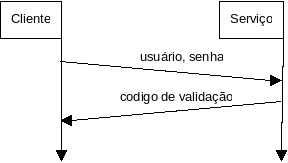
\includegraphics[height=3cm]{img/cap2/autenticacao.png}
\centering

Fonte: Adaptado de ~\cite{LeckyThompson2008Nov}
\end{figure}



Esse método de autenticação é definido pela RFC7519~\cite{rfc7519}, com a tecnologia \ac{jwt}.
%
O código de validação repassado é auditorado em qualquer serviço pertencente ao jogo, visto que ele foi assinado pelo sistema de autenticação do serviço~\cite{Ikem2018May}.


Após a autenticação, é comum existir um sistema para seleção de personagem, caso o jogo seja desenhado com este objetivo.
%
Efetuada a seleção ou criação de um personagem, ele será imerso no mundo compartilhado do jogo com os demais jogadores~\cite{matthiasrudy2011}.


\begin{figure}[htb!]
\caption{Área de interesse com base na proximidade de um jogador}
\label{fig:proximidade}
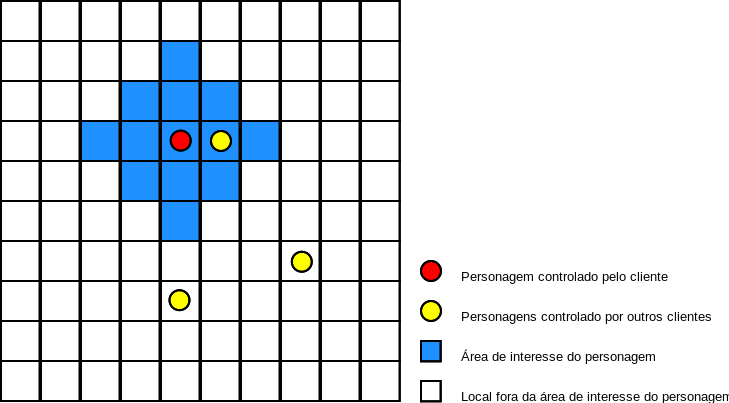
\includegraphics[height=3.8cm]{img/cap2/proximidade.png}
\centering

Fonte:~\cite{albion_online_unite}
\end{figure}



Nos jogos \ac{mmorpg} é comum a restrição da visão do personagem, ora pelas características de jogabilidade do gênero \ac{mmorpg} ora por motivos de desempenho e otimização.
%
Como o jogador não precisa obter dados de regiões que não estão em sua área de interesse, não há necessidade da transmissão de informações dos objetos que estão fora desse contexto~\cite{albion_online_unite}.
%
Esse caso pode ser visualizado na Figura \ref{fig:proximidade}, na qual o personagem selecionado (destacado em vermelho) tem uma área de interesse de baixa distância e uma área de interesse de longa distância~\cite{albion_online_unite}, sendo que o jogador não tem informações de demais objetos e jogadores fora de sua área de interesse.
%
Esta característica impede trapaças (visto que o cliente não tem informações que só estão contidas no serviço) e reduz a frequência de atualização a cada cliente~\cite{albion_online_unite}.



Algumas ações comuns dentro do ambiente de um jogo \ac{mmorpg}~\cite{mmorpg_culture}:

\begin{itemize}
  \item Enviar e receber mensagem no chat;
  \item Mover-se pelo ambiente;
  \item Interagir com outros jogadores, \ac{npcs} ou objetos fixos do ambiente; e
  \item Obter itens do ambiente.
\end{itemize}



O envio e recepção de mensagens do chat é dado com o contexto do posicionamento do personagem~\cite{albion_online_unite}, visível na Figura \ref{fig:chat}.
%
Somente outros personagens dentro de uma distância podem receber alguma mensagem emitida pelo jogador $P_n$.



Essa distância pode ser calculada utilizando Distância Euclidiana~\cite{Deza2009Aug}, na qual a distância entre dois personagens podem ser calculadas pela equação $d(p, q) = \sqrt{\sum_{i=1}^{n}(q_i - p_i)^2}$.
%
Para diminuir a complexidade das comparações a fim de decidir quais personagens $P_n$ devem receber a mensagem, é comum utilizar técnicas de divisão de área utilizando algoritmos como \textit{Quadtree} ou \textit{Octree}~\cite{Lengyel2011Jun}, subdividindo os quadrantes de uma região do ambiente do jogo a fim de facilitar a consulta de quais personagens estão em determinada área deste ambiente.


\begin{figure}[htb!]
\caption{Chat baseado em contexto de posicionamento, utilizando Distância Euclidiana}
\label{fig:chat}
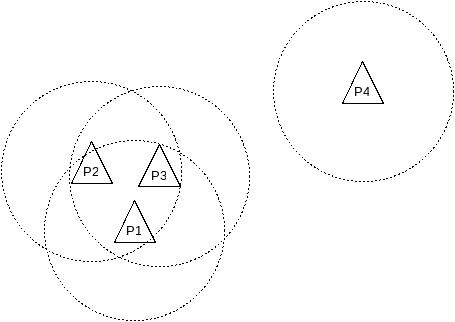
\includegraphics[height=8cm]{img/cap2/chat.png}
\centering

Fonte: Adaptado de ~\cite{albion_online_unite}
\end{figure}



Nesse sentido, a Figura~\ref{fig:chat} mostra a interseção entre o raio de quatro personagens.
%
Nesse exemplo, Mostra-se visível que a as mensagens de $P_1$ devem ser visíveis a $P_2$ e $P_3$, mas não a $P_4$, caso seja utilizado a Distância Euclidiana como regra de distância.



O sistema de movimento pelo ambiente do jogo possibilita que cada jogador movimente o seu personagem a fim de explorá-lo.
%
Dessa maneira, este é um sistema crítico para um jogo \ac{mmorpg}, visto que este sistema será utilizado para inúmeras consultas de proximidade, além de ter uma frequência de atualização e consultas pelos jogadores muito frequente~\cite{albion_online_unite}.


\begin{figure}[htb!]
\caption{Personagens e os seus pontos de destino}
\label{fig:walk}
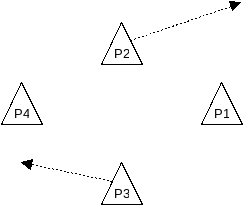
\includegraphics[height=4cm]{img/cap2/walk.png}
\centering

Fonte: Elaborado pelo Autor
\end{figure}



Para os demais sistemas como combate, interação com o mundo, jogadores ou \ac{npcs} também utiliza-se do sistema de raio máximo de interação~\cite{albion_online_unite}.
%
Este sistema não permite o personagem interagir com objetos que não estão dentro do contexto de seu posicionamento no ambiente~\cite{albion_online_unite}.


Essas operações precisam de desempenho para não causar frustração ao jogador final~\cite{7008965}.
%
Nesse sentido, torna-se necessário conhecer os problemas computacionais conhecidos com relação aos serviços de jogos \ac{mmorpg}.

\section{Problemas em jogos MMORPG}
\label{sec:problemas}

Uma métrica popular para mensurar o desempenho de um serviço \ac{mmorpg} é o número de conexões~\cite{1417630} simultâneas suportadas.
%
Em geral, caso o serviço ultrapasse o limite para o qual este foi projetado, diversas falhas de conexão, problemas de lentidão ou dessincronização com o cliente podem ocorrer.
%
Neste contexto, as ocorrências comuns são~\cite{1417630}:

\begin{itemize}
  \item \textbf{Longo tempo de resposta aos clientes}: implica em uma qualidade insatisfatória de jogabilidade ao usuário ou até mesmo impossibilitando o uso do serviço.
  \item \textbf{Dessincronização com os clientes}: realiza reversão na aplicação. Reversão é definida pela situação na qual uma requisição é solicitada ao servidor, um pré-processamento aparente é executado e essa requisição é negada, sendo necessário desfazer o pré-processamento aparente realizado ao cliente.
  \item \textbf{Problemas internos ao serviço}:  podem estar relacionados a diversos outros erros internos de implementação ou a capacidade de recurso computacional (\textit{e.g.,} sobrecarga no banco de dados, gerenciamento lento do espaço ou inconsistências dentro do jogo perante a regra de negócios).
  \item \textbf{Falha de conexão entre o cliente e o serviço}: causa a negação de serviço ao usuário final.
\end{itemize}

Existem algumas causas comuns para essas as ocorrências descritas~\cite{1417630}:

\begin{itemize}
  \item \textbf{Baixo poder computacional do servidor}: poder computacional baixo para a qualidade de experiência de jogabilidade do usuário final desejada.
  \item \textbf{Complexidade de algoritmos}: o serviço usa algoritmos de alta complexidade ou regras de negócios que demandam por um algoritmo complexo.
  \item \textbf{Limitado pela própria arquitetura}: está limitado diretamente pelo número de conexões, não suportando a carga recebida.
\end{itemize}

Tais ocorrências estão diretamente correlacionadas a carga a qual tais serviços estão submetidos e podem ser amenizadas utilizando técnicas de provisionamento de recursos e balanceamento de carga~\cite{1417630}, mas não suficiente para eliminar tais ocorrências.

A área de desenvolvimento web compartilha várias ocorrências comuns geradas por sobrecarga do serviço~\cite{7830692}.
%
Em desenvolvimento web é comum utilizar a abordagem de microsserviços para resolver o problema de sobrecarga, modularizando o  funcionamento em módulos menores.
%
Da mesma forma, faz sentido modularizar um serviço \ac{mmorpg} em microsserviços para suportar cargas maiores e diminuir o custo de manutenção~\cite{7515686}.


Do ponto de vista da arquitetura de computadores, as operações existentes em um jogo \ac{mmorpg} seguem um padrão de interação com o mundo, criar, excluir ou manipular objetos deste mundo.

%
Para suprir o desenvolvimento de tais sistemas, se faz necessário compreender os padrões de desenvolvimento de tais arquiteturas na qual suprem as operações básicas de interação com o mundo.


\section{Arquitetura de Clientes MMORPG}
\label{sec:cliente}



Do ponto de vista da rede de computadores, a arquitetura de um cliente de jogo \ac{mmorpg} deve suportar consultas e chamadas de métodos remotos em um serviço~\cite{albion_online_unite}.
%
Um cliente para um jogo \ac{mmorpg} segue o estilo de arquitetura \ac{rest}, porém não obrigatoriamente sobre o protocolo \ac{http}.
%
A fim de reduzir o custo operacional das requisições, as consultas podem ser escritas sobre um protocolo otimizado conveniente a aplicação na camada de transporte (\textit{e.g.,}, \ac{tcp}, \ac{udp}, etc)~\cite{albion_online_unite, stephenclarkewillson2017}.

O módulo de \textit{Gateway}, implementado dentro de um cliente de jogo \ac{mmorpg}, é responsável por realizar as requisições ao servidor e aplicar as chamadas de métodos internas ao cliente para exibir o estado de jogo ao jogador~\cite{albion_online_unite}.
%
Ele pode ser encontrado na Figura \ref{fig:gateway}.


\begin{figure}[htb!]
\caption{Requisição de uma chamada de método pela visão do cliente.}
\label{fig:gateway}
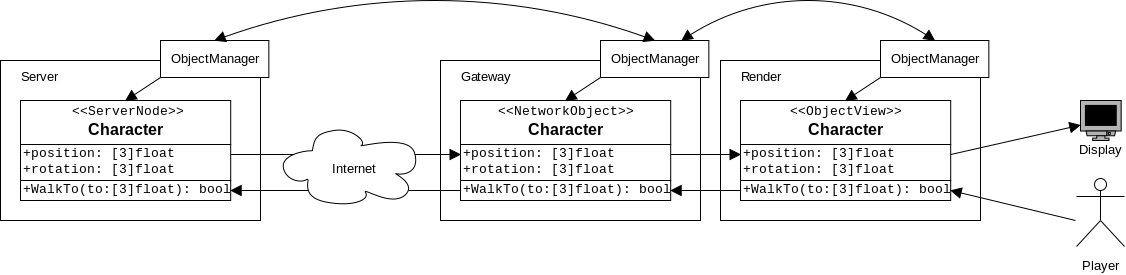
\includegraphics[height=3.8cm]{img/cap2/gateway.png}
\centering

Adaptado de:~\cite{albion_online_unite}
\end{figure}



A Figura \ref{fig:gateway} refere-se a uma visão macro de uma requisição realizada pelo jogador.
%
Nessa requisição, o jogador realiza o pedido para o seu personagem caminhar até um determinado ponto.
%
Essa requisição será processada pelo servidor, que atualizará sua posição e retornará ao Gateway a nova posição do personagem, exibindo o personagem em uma nova posição.



Para facilitar o desenvolvimento, a aplicação de cliente é dividida em diversos módulos, sendo os dois principais~\cite{albion_online_unite}:



\begin{itemize}
  \item \textbf{Renderização:} É o processo que transformará a estrutura de dados obtida do serviço de forma gráfica ao jogador utilizando um motor gráfico (\textit{e.g.,} Unity3D\footnote{Unity3D: \url{https://www.unity3d.com}}, GodotEngine\footnote{GodotEngine: \url{https://www.godotengine.org}}, etc).
  \item \textbf{Gateway:} É o módulo responsável pela comunicação entre o serviço e o cliente, a fim de requisitar chamadas de métodos ou obter informações do servidor.
\end{itemize}



Também existe um módulo nomeado \textit{ObjectManager} na Figura \ref{fig:gateway} que gerenciará a criação e deleção de objetos do mundo.
%
Tanto os objetos em cena quanto o ObjectManager podem ser utilizados ora pelo jogador ora pelo serviço a fim de sincronizar o cliente ou realizar requisições ao serviço.
%
Entretanto, existe um filtro de requisições maliciosas a fim de garantir a consistência do jogo~\cite{albion_online_unite}.
%
Esse filtro pode ser implementado no Gateway e/ou no serviço (Seção \ref{sec:arquiteturas}).



Uma característica importante do ObjectManager é a requisição e exibição de objetos com base na área de interesse do jogador.
%
Essa característica reduz problemas de trapaça por meio de clientes adulterados (visto que limita a interação de objetos do cliente) e reduz o tráfego de dados na rede tanto para o cliente quanto para o serviço~\cite{albion_online_unite, stephenclarkewillson2017}.



A abordagem de engenharia por utilizar um Gateway permite que o serviço mude de arquitetura sem a necessidade de uma refatoração completa ao módulo de renderização~\cite{albion_online_unite, stephenclarkewillson2017}.
%
Essa mesma abordagem também facilita o desenvolvimento de uma suíte de testes do módulo de renderização independente do serviço~\cite{Freeman2009Oct}, podendo realizar testes utilizando o padrão de objetos Mock~\cite{Beck2004Nov} para simular as requisições.
%
Dessa forma, é possivel garantir um padrão de integração desejado entre o serviço e o cliente utilizando baixo acoplamento, com ganho de desempenho na suíte de testes do cliente, sem a necessidade real de um serviço para testar o cliente.



\section{Arquitetura de Microsserviços}
\label{sec:microsservicos}



Entende-se por microsserviço aplicações que executam operações menores de um macrosserviço, da melhor forma possível~\cite{stephenclarkewillson2017, Newman2015Feb}.
%
O objetivo de uma arquitetura de microsserviços é funcionar separadamente de forma autônoma, contendo baixo acoplamento~\cite{Newman2015Feb}.
%
Seu funcionamento deve ser desenhado para permitir alinhamentos de alta coesão e baixo acoplamento entre os demais microsserviços existentes em um macrosserviço~\cite{8169955}.



Arquiteturas de microsserviços iniciam uma nova linha de desenvolvimento de aplicações preparadas para executar sobre nuvens computacionais, promovendo maior flexibilidade, escalabilidade, gerenciamento e desempenho, sendo a principal escolha de arquitetura de grandes empresas como Amazon, Netflix e LinkedIn~\cite{7830692,7515686}.
%
Um microsserviço é definido pelas seguintes características~\cite{8169955}:



\begin{itemize}
  \item Deve possibilitar a implementação como uma peça individual do macrosserviço.
  \item Deve funcionar individualmente.
  \item Cada serviço deve ter uma interface. Essa interface deve ser o suficiente para utilizar o microsserviço.
  \item A interface deve estar disponível na rede para chamada de processamento remoto ou consulta de dados.
  \item O serviço pode ser utilizado por qualquer linguagem de programação e/ou plataforma.
  \item O serviço deve executar com as dependências mínimas.
  \item Ao agregar vários microsserviços, o macrosserviço resultante poderá prover funcionalidades complexas.
\end{itemize}

%ccm 23
\begin{figure}[htb!]
\caption{Microsserviços podem ter diferentes tecnologias}
\label{fig:microsservicos_tecnologias}
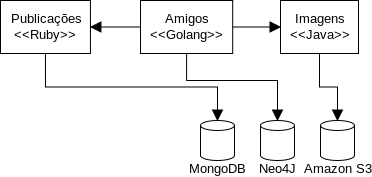
\includegraphics[height=4cm]{img/cap2/microsservicos_tecnologias.png}
\centering

Adaptado de:~\cite{Newman2015Feb}
\end{figure}

%ccm 24
O microsserviço deverá ser uma entidade separada. Ela deve ser implantada como um sistema independente em um \ac{paas}.
%
Toda a comunicação entre os microsserviços de um macrosserviço será executada sobre a rede, a fim de reforçar a separação entre cada serviço.
%
As chamadas pela rede com o cliente ou entre os microsserviços será executada através de uma \ac{api}, permitindo a liberdade de tecnologia em que cada um será implementado~\cite{Newman2015Feb}.



\begin{figure}[htb!]
\caption{Microsserviços são escaláveis}
\label{fig:microsservicos_escalabilidade}
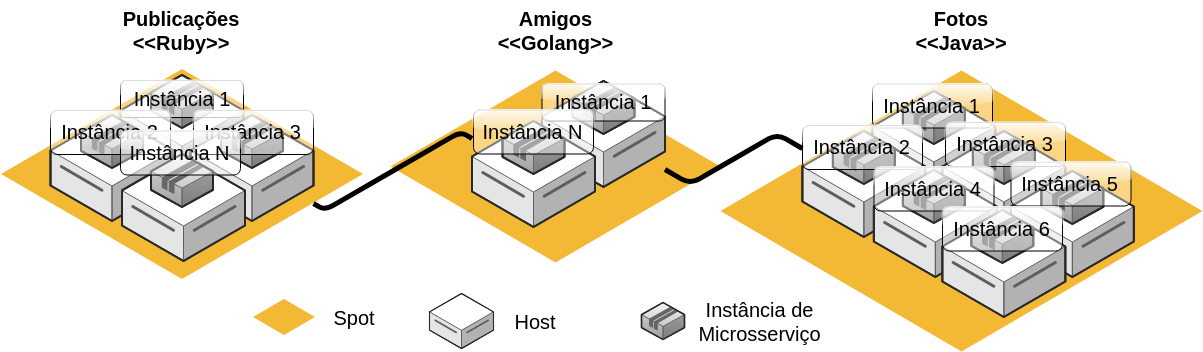
\includegraphics[height=5cm]{img/cap2/microsservicos_escalabilidade.png}
\centering

Adaptado de:~\cite{Newman2015Feb}
\end{figure}



Uma arquitetura de microsserviços é escalável, como visível na Figura \ref{fig:microsservicos_escalabilidade}.
%
Ela permite o aumento do número de microsserviços sob demanda para suprir a necessidade de escalabilidade.
%
Este modelo computacional obtém maior desempenho, principalmente se executar sobre plataformas de computação elástica, na qual o orquestrador do macrosserviço pode aumentar o número de instâncias conforme a necessidade de requisições~\cite{Nadareishvili2016Aug}.



Microsserviços desenvolvidos para web utilizam arquitetura \ac{rest} baseado sobre o protocolo \ac{http}.
%
É uma boa prática utilizar o corpo com conteúdo da requisição e resposta no formato \ac{json} nas chamadas a uma \ac{api} de microsserviço web~\cite{Nadareishvili2016Aug}.



Entretanto não é uma prática comum para um serviço \ac{mmorpg} utilizar o protocolo \ac{http} pela sua elevada carga desnecessária na requisição~\cite{1417630}.
%
Por esse motivo se faz necessário ver as diferenças entre uma arquitetura de microsserviços para \ac{mmorpg} comparados a microsserviços web.



\subsection{Protocolos para microsserviços \ac{mmorpg}}



Um serviço \ac{mmorpg} não utilizará protocolos com base no protocolo \ac{http}, mas ainda assim implementará um protocolo \ac{rest} sobre o protocolo \ac{tcp} a fim de realizar requisições a um serviço utilizando uma arquitetura de software \ac{mvc}~\cite{Chadwick2012Oct, LeckyThompson2008Nov}.
%
O protocolo \ac{rest} permitirá ele, similar a técnica de armazenamento persistente \ac{crud}, executar quatro métodos aos controladores de cada microsserviço~\cite{6267019}:



\begin{enumerate}
  \item Criar: Permite criar um dado no serviço (\textit{e.g.,} criar um personagem em sua conta, criar um pedido de amizade, etc).
  \item Ler: Permite consultar um dado no serviço (\textit{e.g.,} ler os personagens que estão em sua região, ler os itens, etc).
  \item Atualizar: Permite atualizar um dado no serviço (\textit{e.g.,} efetuar a compra de um item de \ac{npcs}, andar para um ponto do mapa, etc).
  \item Deletar: Permite deletar um dado no serviço (\textit{e.g.,} usar um item do inventário, deletar uma mensagem lida de um amigo, etc).
\end{enumerate}



Porém, além de realizar as operações \ac{crud}, se faz necessário a chamada de métodos específicos a um objeto.
%
Pode-se associar a técnica de \ac{rpc}~\cite{LeckyThompson2008Nov}. Pode-se analisar um exemplo da interface disponível na Figura \ref{fig:crud_rpc} e o diagrama de requisições na Figura \ref{fig:network_crud_rpc}.



\begin{figure}[htb!]
\caption{Cliente pode realizar requisições \ac{crud} ou \ac{rpc}}
\label{fig:crud_rpc}
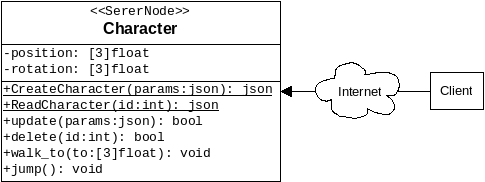
\includegraphics[height=4.5cm]{img/cap2/crud_rpc.png}
\centering

Fonte: Elaborado pelo autor
\end{figure}



\begin{figure}[htb!]
\caption{Diagrama de requisições entre serviço e cliente com operações \ac{crud} e \ac{rpc} em uma arquitetura monolítico}
\label{fig:network_crud_rpc}
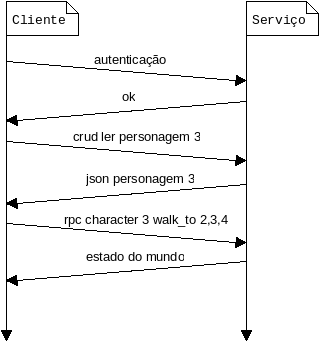
\includegraphics[height=6.5cm]{img/cap2/network_rpc_crud.png}
\centering

Fonte: Adaptado de~\cite{LeckyThompson2008Nov}
\end{figure}



Uma técnica comum em jogos é a compressão de pacotes utilizando mapeamento hash de bytes~\cite{LeckyThompson2008Nov}.
%
Tanto o cliente quanto o serviço precisam ter a mesma estrutura de dados.
%
Dessa forma, é possivel trocar o nome das funções requiridas em \ac{rpc} por poucos bytes para transitar na rede.
%
Já para operações \ac{crud}, pode-se utilizar tanto requisições sobre o protocolo \ac{http} ou sobre um protocolo otimizado sobre \ac{tcp} dependendo da necessidade de desempenho~\cite{LeckyThompson2008Nov}.

Como relatado na Seção \ref{sec:microsservicos}, uma arquitetura de microsserviços permite multiplas tecnologias, pois a comunicação entre todos os elementos de um microsserviço será pela rede.
%
Por esse motivo, é possível utilizar um serviço web para realizar operações \ac{crud} e um serviço dedicado para realizar operações \ac{rpc}.
%
Essa arquitetura pode ser melhor compreendida pela Figura \ref{fig:network_crud_rpc_micro}.



\begin{figure}[htb!]
\caption{Diagrama de requisições entre serviço e cliente com operações \ac{crud} e \ac{rpc} em uma arquitetura de microsserviços}
\label{fig:network_crud_rpc_micro}
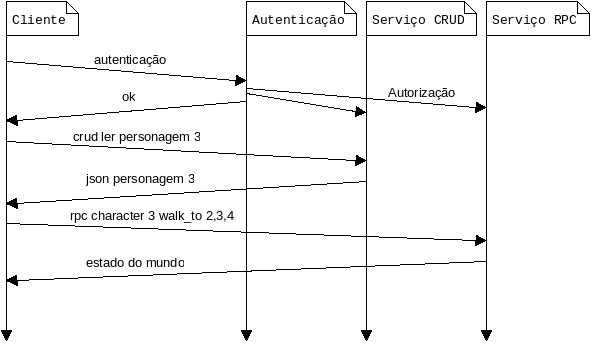
\includegraphics[height=6.5cm]{img/cap2/network_rpc_crud_micro.png}
\centering

Fonte: Elaborado pelo Autor
\end{figure}



Utilizando esse embasamento teórico sobre microsserviços e arquiteturas de jogos \ac{mmorpg}, pode-se analisar os trabalhos (Seção \ref{sec:similares}) relacionados com o tema proposto no atual documento.



\section{Trabalhos Relacionados}
\label{sec:similares}



Para nortear o desenvolvimento da análise se microsserviços utilizados em jogos \ac{mmorpg} proposto no atual trabalho, essa seção apresenta outros trabalhos que têm o escopo ou objetivo similar, no qual monitoraram e analisaram serviços de jogos \ac{mmorpg}.
%
Ao apresentar estes trabalhos, busca-se apresentar o contexto e objetivo, e então aprofundar em características, métricas e ferramentas que auxiliaram nas análises.
%
%Por fim, será necessário apresentar na Seção \ref{sec:similares_analise} uma análise das abordagens e resultados obtidos dos trabalhos relacionados.



\subsection{Huang et al. (2004)}
\label{sec:huang}


O trabalho de ~\cite{1417630} investiga a relação entre os recursos utilizados e o número de conexões presentes em um serviço \ac{mmorpg} distribuído.
%
Neste trabalho é relatado que a infraestrutura utiliza três serviços: Um \textit{Game Server} sobre protocolo \ac{tcp}, um \textit{Proxy Server} também sobre protocolo \ac{tcp}, e um servidor web para autenticação que executa sobre uma interface \ac{http}.
%
O foco de análise é o \textit{Game Server} e o \textit{Proxy Server}.



\begin{figure}[htb!]
\caption{Arquitetura distribuída utilizando proxy}
\label{fig:game_with_proxy}
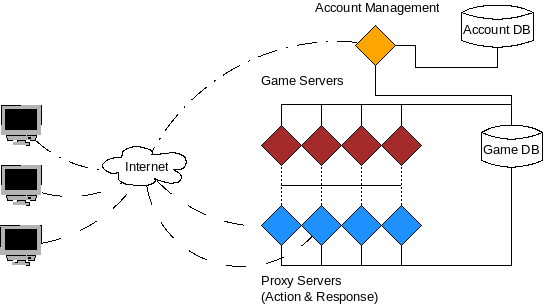
\includegraphics[height=7cm]{img/cap2/game_with_proxy.png}
\centering

Adaptado de:~\cite{1417630}
\end{figure}



A infraestrutura do servidor de jogo contém um \textit{Proxy Server Farm} utilizando o algoritmo \textit{Round Robin} com pesos para balanceamento de carga entre cada cliente.
%
Cada \textit{Proxy Server} é responsável por comunicar com os demais microsserviços privados ao servidor, baseado com a área de interesse de sua conexão.
%
O protocolo de comunicação utilizado entre o Cliente e \textit{Proxy Server} é baseado em \ac{rpc}~\cite{faber, borella}, porém não é relatado sobre o o protocolo de comunicação utilizado entre o \textit{Proxy Server} e o \textit{Game Server}.
%
A sua arquitetura pode ser observada na Figura \ref{fig:game_with_proxy}, na qual obteve seus dados obtidos durante 100 dias para realizar as análises.
%
A Figura \ref{fig:players_peer_time} demonstra uma amostra do número de conexões pelo tempo no serviço obtido.



\begin{figure}[htb!]
\caption{Número de conexões no serviço pelo tempo decorrido}
\label{fig:players_peer_time}
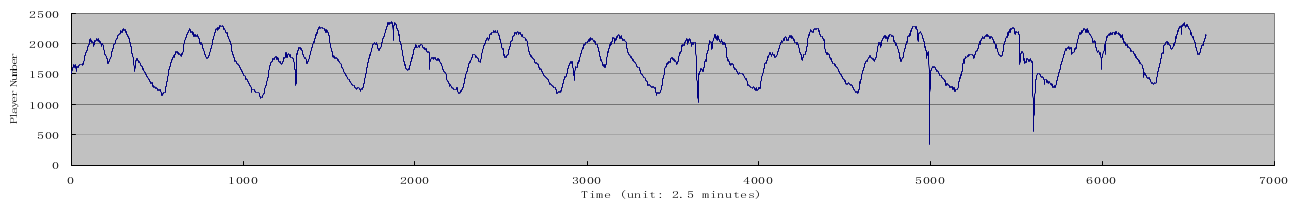
\includegraphics[height=2.5cm]{img/cap2/players_peer_time.png}
\centering

Fonte:~\cite{1417630}
\end{figure}



Como análise, o autor correlacionou o número de conexões com número de pacotes, banda, memória e \ac{cpu} consumidos utilizando uma função estatística linear.
%
Esta função pode ser utilizada com regressão linear para prever consumo de recursos futuros e por fim realocar mais recursos ao serviço, contribuindo com escalabilidade vertical autônoma.
%
Um exemplo de aplicação dessa regressão linear pode ser visualizada na Figura~\ref{fig:regressao_bytes}, onde o autor compara o consumo de banda real comparado a regressão linear.


\begin{figure}[htb!]
\caption{Regressão linear comparado ao consumo de banda real do servidor}
\label{fig:regressao_bytes}
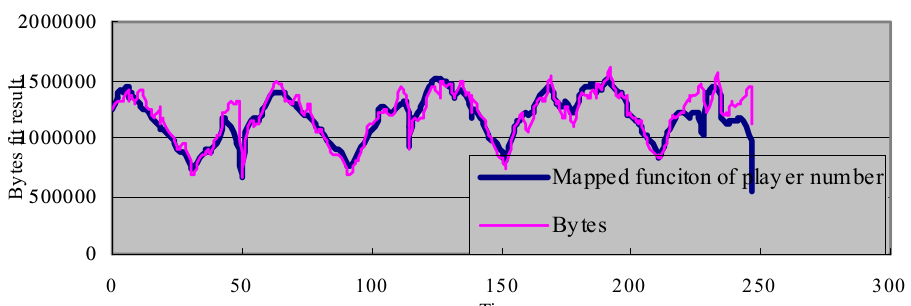
\includegraphics[height=4.5cm]{img/cap2/regressao.png}
\centering

Fonte:~\cite{1417630}
\end{figure}


Entretanto, a escalabilidade horizontal não pode ser prevista, visto que não é analisado o posicionamento de cada personagem a fim de dividir os ambientes em pedaços menores com outros serviços.
%
Como trabalhos futuros é relatado a análise do posicionamento de personagens para escalabilidade horizontal, a análise de outras arquiteturas e timos de jogos diferentes e qual o impácto de utilizar balanço de carga e provisionamento de recursos de forma dinâmica.



\subsection{Villamizar et al. (2016)}



O trabalho de ~\cite{7515686} investiga o custo de arquiteturas de microsserviços, arquiteturas \ac{paas} orientedas a eventos e aplicações monolíticas para aplicações web.
%
A sua principal motivação é a comparação de custos para a tradução de sistemas legados para arquiteturas distribuídas.
%
Para isso, o autor preparou 3 instâncias de testes com suas configurações desenhadas a fim de ter o maior número de requisições por minuto com o mesmo custo financeiro.



\begin{figure}[htb!]
\caption{Arquitetura monolítica web implementada na \ac{aws}}
\label{fig:aws_monolitico}
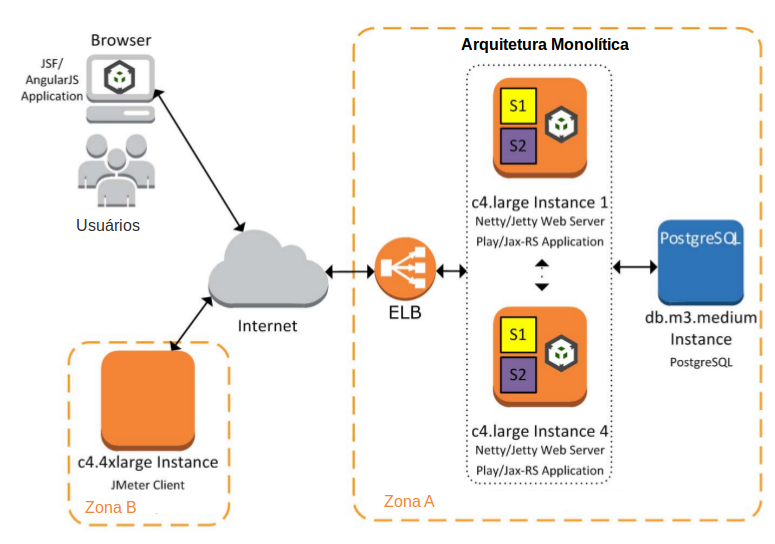
\includegraphics[height=4.5cm]{img/cap2/aws_monolitico.png}
\centering

Fonte:~\cite{7515686}
\end{figure}

\textbf{Instância I.} Utilizando quatro instâncias \ac{aws} \textit{c4.large}, uma instância \ac{aws} \textit{c4.xlarge} e uma instância \ac{aws} \textit{db.m3.medium}..
%
A Figura~\ref{fig:aws_monolitico} exibe a implantação de uma aplicação web monolítica.
%
Essa arquitetura foi implementada utilizando \textit{Jax-RS} e \textit{Play Framework}.




\begin{figure}[htb!]
\caption{Arquitetura de microsserviços web implementada na \ac{aws}}
\label{fig:aws_microsservicos}
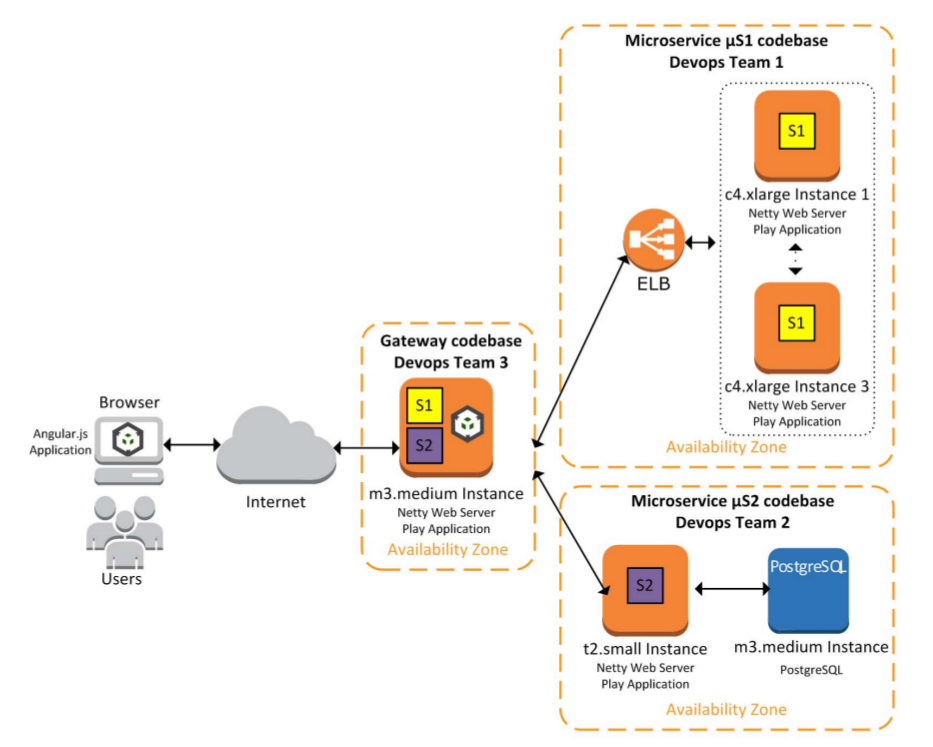
\includegraphics[height=4.5cm]{img/cap2/aws_microsservicos.png}
\centering

Fonte:~\cite{7515686}
\end{figure}

\textbf{Instância II.} Utilizando três instâncias \ac{aws} \textit{c4.xlarge}, uma instância \ac{aws} \textit{t2.small} e uma instância \ac{aws} \textit{db.m3.medium}.
%
A Figura~\ref{fig:aws_microsservicos} exibe a implantação de uma aplicação de microsserviços web. Essa arquitetura foi implementada utilizando \textit{Play Framework}.



\begin{figure}[htb!]
\caption{Arquitetura de microsserviços web implementada na \ac{aws} utilizando a tecnologia \textit{lambda}}
\label{fig:aws_lambda}
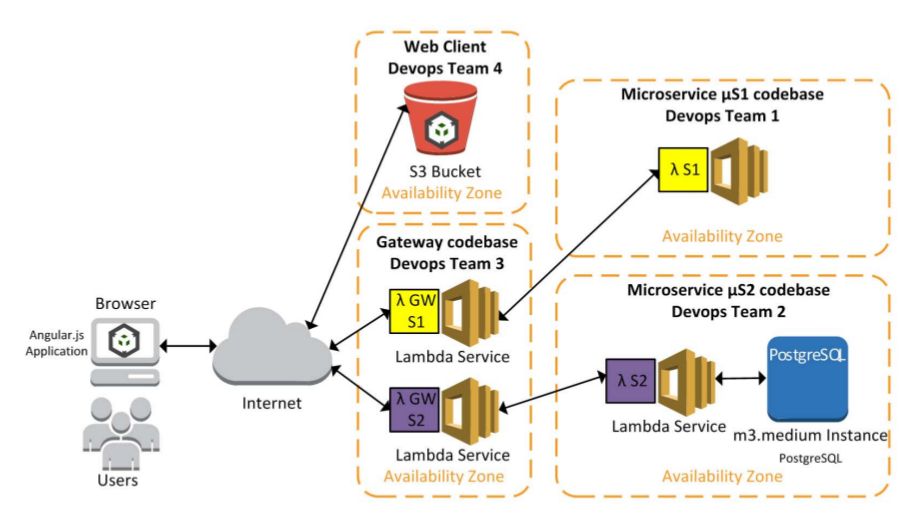
\includegraphics[height=4.5cm]{img/cap2/aws_lambda.png}
\centering

Fonte:~\cite{7515686}
\end{figure}

\textbf{Instância III.} Utilizando duas instâncias \ac{aws} \textit{lambda S1}, duas instâncias \ac{aws} \textit{lambda S2}, uma instância \ac{aws} \textit{S3 Bucket} e uma instância \ac{aws} \textit{db.m3.medium}.
%
A Figura~\ref{fig:aws_lambda} exibe a implantação de uma aplicação de microsserviços web utilizando a tecnologia \ac{aws} \textit{lambda}. Essa arquitetura foi implementada em \textit{Node.js}, onde as funções de \textit{gateway} foram implementadas em quatro funções independentes do tipo \textit{microservice-http-endpoint}.



\begin{figure}[htb!]
\caption{Custo por por um milhão de requisições em dólares utilizando diferentes arquiteturas sobre a \ac{aws}}
\label{fig:custo_aws}
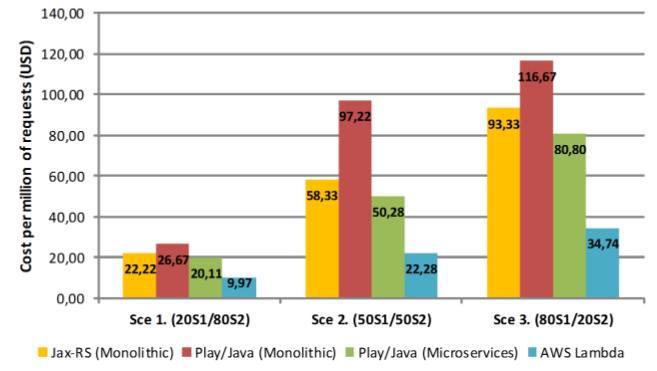
\includegraphics[height=4.5cm]{img/cap2/custo_aws.png}
\centering

Fonte:~\cite{7515686}
\end{figure}



Foi concluído que a arquitetura de microsserviços, nas condições desta aplicação, podem reduzir até 13.42\% em gastos com a infraestrutura.
%
Essa redução pode ser observada na Figura~\ref{fig:custo_aws}.
%
O autor alerta sobre tolerância a falhas, transações distribuidas, distribuição de dados e versionamento de serviço.


\subsection{Suznjevic e Matijasevic (2012)}



O trabalho de ~\cite{6374456} tem seu objetivo a fim de prever a carga a qual um serviço \ac{mmorpg} pode receber utilizando a complexidade das operações nos contextos de \ac{pvp} e \ac{pvnpc} a qual um personagem pode realizar em um ambiente.
%
Este trabalho usa com base o modelo descrito na Sessão~\ref{sec:huang}, um modelo distribuído em serviços na qual efetuam o processamento de uma região do ambiente virtual.



\begin{table}[htb!]
\centering
\caption{Complexidade da interação com o ambiente, por contexto da interação}
\label{tab:complexidade}
\begin{tabular}{|l|l|l|l|l|}
\hline
Contexto da ação        & \ac{pvp}           & \ac{pvnpc}              & Number of \ac{npcs}    & Network {[}kbits/s{]} \\ \hline
Questing                & $O(n)$             & $O(n log(n))$           & $N \leq 6 $            & 11.4          \\ \hline
Trading                 & $O(n)$             & $O(n)$                  & $N \leq 20$            & 8.1           \\ \hline
Dungeons                & $O(n^2)$           & $O(n^2)$                & $N \leq 20$            & 18.3          \\ \hline
\ac{pvp} combat         & $O(n^3)$           & $O(n)$                  & $N = 0    $            & 24.1          \\ \hline
Raiding                 & $O(n^2 log(n))$    & $O(n^3)$                & $N \leq 40$            & 32.0          \\ \hline
\end{tabular}

Fonte:~\cite{6374456}
\end{table}



A análise realizada leva em conta a complexidade das ações no ambiente, a qual pode ser descrita na Tabela~\ref{tab:complexidade}.
%
Essa tabela exibe as ações que podem ser executadas para interagir com o ambiente, seja essa interação com \ac{pvp} (jogador com outro jogador) ou \ac{pvnpc} (jogador com um personagem ou objeto gerenciado pelo serviço).
%
Os contextos analisados nessa tabela são:

\begin{itemize}
  \item \textit{Questing}: Contexto de missão, na qual um grupo de jogadores ou um grupo de \ac{npcs} podem ser afetados nas ações.
  \item \textit{trading}: Contexto de negociação, na qual a complexidade leva em conta somente o número de itens negociados.
  \item \textit{Dungeons}: Contexto de exploração, na qual o ambiente pode ser modificado conforme as ações dos personagens em um ambiente isolado para este grupo.
  \item \textit{\ac{pvp} combat}: Contexto de batalha entre jogadores, na qual as ações entre os jogadores influenciam diretamente o estado do personagem oponente.
  \item \textit{Raiding}: Representa um contexto específico de exploração, onde multiplos jogadores unem forças a fim de combater outro grupo de jogadores ou \ac{npcs}.
\end{itemize}


\begin{figure}[htb!]
\caption{Regressão levando em conta a complexidade das ações e contexto dos personagens}
\label{fig:regressao_complexidade}
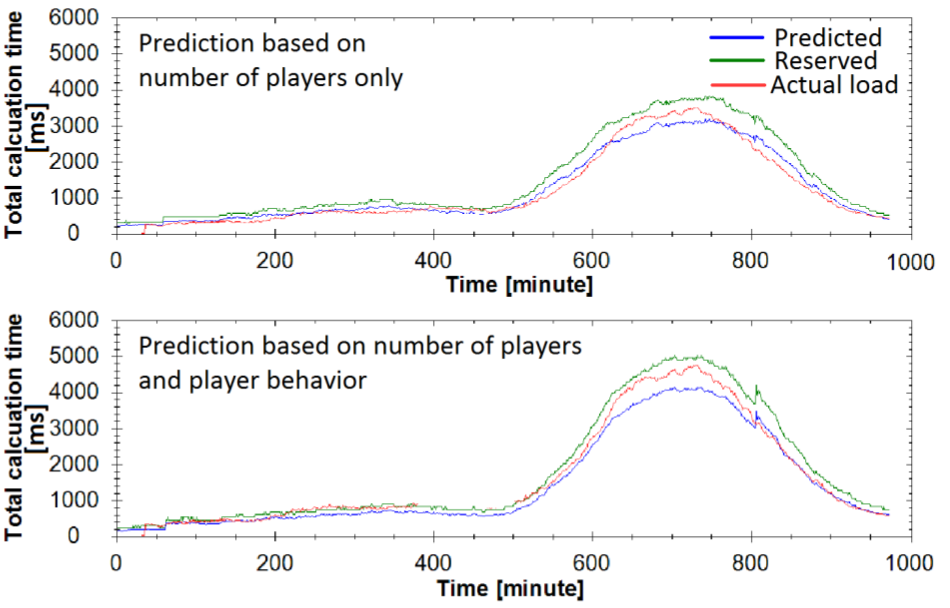
\includegraphics[height=6.0cm]{img/cap2/network_regressao_complexidade.png}
\centering

Fonte:~\cite{6374456}
\end{figure}



Utilizando as complexidades das ações, o número de conexões e o contexto de cada personagem no ambiente para predizer a banda utilizada.
%
Pode-se visualizar uma regressão na Figura~\ref{fig:regressao_complexidade}.



O autor conclui que o contexto de interação com o ambiente de cada personagem tem relevância com o consumo de \ac{cpu} e banda, a qual pode ser calculada com sua complexidade a fim de desenvolver uma ferramenta para predição de carga sobre serviços \ac{mmorpg}.
%
Entretanto, essa predição não é feita em tempo real, não contribuindo para a automação da escalabilidade vertical e horizontal da arquitetura de microsserviços.



\subsection{Análise dos trabalhos relacionados}
\label{sec:similares_analise}
